\subsection{\texorpdfstring{\nitrogen{}}{15N} HMQC}
\label{subsec:noah__hmqc}

In \cref{subsec:noah__sehsqc_n}, I will discuss how the sensitivity-enhanced HSQC modules developed above may be adapted into \proton{}--\nitrogen{} experiments.
However, before that, I make a slight detour to cover the \nitrogen{} HMQC experiment, which (up until my DPhil) was the experiment of choice for detecting one-bond \proton{}--\nitrogen{} correlations.

\begin{figure}[htb]
    \centering
    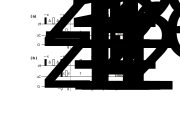
\includegraphics[draft=false]{pp/hmqc/all.png}%
    {\phantomsubcaption\label{fig:noah_hmqc_2grad}}%
    {\phantomsubcaption\label{fig:noah_hmqc_4grad}}%
    \caption[NOAH HMQC pulse sequences]{
        \textbf{(\subref*{fig:noah_hmqc_2grad})} With two encoding gradients around $t_1$.
        \textbf{(\subref*{fig:noah_hmqc_4grad})} With four encoding gradients around $t_1$.
        Phase cycling is performed with $\phi_1 = (x, -x)$, $\phi_2 = (x, x, -x, -x)$, and $\phi_\text{rec} = (x, -x, -x, x)$.
        The delay $\Delta$ is set to $1 / (4 \cdot \oneJ{NH})$.
        Gradient amplitudes are: $g_1 = 80\%$; $g_2 = \pm 32.4\%$; $g_2' = g_2/2$.
    }
    \label{fig:noah_hmqc}
\end{figure}

The HMQC module is based on the ASAP-HMQC reported by Kup{\v{c}}e and Freeman\autocite{Kupce2007MRC}, which used a symmetric gradient scheme similar to that in the seHSQC modules previously described (\cref{fig:noah_hmqc_2grad}).
However, in the NOAH module\autocite{Kupce2017ACIE}, bipolar gradient pulse pairs were placed before and after $t_1$ (\cref{fig:noah_hmqc_4grad}).
This was likely implemented in order to allow the final gradient, $g_2$, to have as large an amplitude as possible.
In heteronuclear experiments, this final gradient is particularly important for dephasing bulk magnetisation which is transverse just prior to detection (due to pulse imperfections or relaxation).
If this gradient is too weak, this unwanted magnetisation will be incompletely dephased, leading to artefacts in the resulting spectrum.

Strategies to maximise this gradient amplitude are particularly crucial in \proton{}--\nitrogen{} experiments (as compared to \proton{}--\carbon{} experiments) for two reasons.
Firstly, the natural abundance of \nitrogen{} (0.36\%) is even smaller than \carbon{} (1.1\%), meaning that better suppression must be achieved in order for the artefacts to not obscure the signal.
Secondly, the gyromagnetic ratio of \nitrogen{} is also smaller: thus, since $g_2/g_1 \propto \gammaN/\gammaH$, an unmodified pulse sequence will naturally have a smaller $g_2$.

In this respect, the four-gradient scheme in \cref{fig:noah_hmqc_4grad} is superior to the two-gradient scheme, because the gradient $g_2$ will have an amplitude of $4\gammaN g_1/\gammaH$.
However, when used in a NOAH supersequence, this leads to wing artefacts in downstream modules, since bulk \magnnot{N} magnetisation effectively does not experience any coherence order selection during $t_1$.
This motivates a return to the two-gradient scheme of \cref{fig:noah_hmqc_2grad}.
To compensate for the fact that the decoding gradient $g_2'$ has half of the amplitude of $g_2$, all CTP gradients were instead \textit{lengthened} from their usual duration of \qty{1}{\ms} to \qty{2.5}{\ms}.
This ensures that any stray transverse bulk magnetisation at the end of the HMQC module is effectively dephased.

The HMQC spectra thus obtained are shown in \cref{fig:hmqc_grad_spec}.
The first column shows the spectra obtained with the original four-gradient scheme: although the artefacts at \qty{2.2}{\ppm} are reasonably well-suppressed in the HMQC module (\cref{fig:hmqc_grad_spec_4grad_1ms_hmqcp}), the CLIP-COSY spectrum clearly has a set of wing artefacts (\cref{fig:hmqc_grad_spec_4grad_1ms_cosy}).
(Note that the wing artefacts occur at different frequencies compared to the \carbon{} seHSQC case, because the $t_1$ increment in the \nitrogen{} HMQC module is different.)

The second column shows what happens when the two-gradient scheme is adopted without changing the gradient duration.
Although the CLIP-COSY wing artefacts disappear (\cref{fig:hmqc_grad_spec_2grad_1ms_cosy}), the HMQC artefacts are over twice as intense (\cref{fig:hmqc_grad_spec_2grad_1ms_hmqcp}), and (in this case) have comparable intensity to the desired peaks.

By using the two-gradient scheme and increasing the gradient duration to \qty{2.5}{\ms}, we obtain the best of both worlds: the HMQC artefacts are well-suppressed (\cref{fig:hmqc_grad_spec_2grad_2p5ms_hmqcp}, in fact even better than in the original spectrum), and the CLIP-COSY is free of wing artefacts (\cref{fig:hmqc_grad_spec_2grad_2p5ms_cosy}).
The only drawback is a slight loss in signal intensity in the HMQC, which arises due to diffusion and relaxation during the longer pulse sequence.
However, this decrease is only on the order of $5\%$ (for this particular case), which is a totally acceptable price to pay in return for the improved spectral quality.

\begin{figure}[!htbp]
    \centering
    \includegraphics[draft=false]{noah/hmqc_grad.png}%
    {\phantomsubcaption\label{fig:hmqc_grad_spec_4grad_1ms_hmqc}}%
    {\phantomsubcaption\label{fig:hmqc_grad_spec_4grad_1ms_hmqcp}}%
    {\phantomsubcaption\label{fig:hmqc_grad_spec_4grad_1ms_cosy}}%
    {\phantomsubcaption\label{fig:hmqc_grad_spec_2grad_1ms_hmqc}}%
    {\phantomsubcaption\label{fig:hmqc_grad_spec_2grad_1ms_hmqcp}}%
    {\phantomsubcaption\label{fig:hmqc_grad_spec_2grad_1ms_cosy}}%
    {\phantomsubcaption\label{fig:hmqc_grad_spec_2grad_2p5ms_hmqc}}%
    {\phantomsubcaption\label{fig:hmqc_grad_spec_2grad_2p5ms_hmqcp}}%
    {\phantomsubcaption\label{fig:hmqc_grad_spec_2grad_2p5ms_cosy}}%
    \caption[Comparison of \noah{M,Sp,Cc} modules with different HMQC gradient schemes]{
        Comparison of HMQC and CLIP-COSY spectra obtained from \noah{M,Sp,Cc} supersequences, acquired using different HMQC gradient schemes.
        In the first row, the HMQC spectrum itself is shown.
        In the second row, the positive projection of the HMQC spectrum onto the $f_2$ axis is shown; the numbers indicate peak intensities with respect to the reference dataset (the left column).
        The asterisk indicates artefacts arising from bulk magnetisation which is not sufficiently dephased by the final gradient.
        In the third row, (an inset of) the CLIP-COSY spectrum is shown.
        \textbf{(\subref*{fig:hmqc_grad_spec_4grad_1ms_hmqc})--(\subref*{fig:hmqc_grad_spec_4grad_1ms_cosy})} Using the four-gradient scheme of \cref{fig:noah_hmqc_4grad}, with \qty{1}{ms} gradients.
        \textbf{(\subref*{fig:hmqc_grad_spec_2grad_1ms_hmqc})--(\subref*{fig:hmqc_grad_spec_2grad_1ms_cosy})} Using the two-gradient scheme of \cref{fig:noah_hmqc_2grad}, with \qty{1}{ms} gradients.
        \textbf{(\subref*{fig:hmqc_grad_spec_2grad_2p5ms_hmqc})--(\subref*{fig:hmqc_grad_spec_2grad_2p5ms_cosy})} Using the two-gradient scheme of \cref{fig:noah_hmqc_2grad}, with \qty{2.5}{ms} gradients.
        \datacode{7Z-200926}
    }
    \label{fig:hmqc_grad_spec}
\end{figure}

It is of some interest to check whether such a long gradient is truly required.
I therefore ran the two-gradient HMQC experiment with a series of gradient durations from \qty{1}{\ms} to \qty{2.5}{\ms}; the signal and artefact intensities in each of these experiments are plotted in \cref{fig:hmqc_cnst16}.
Generally, there is little variation in the intensities of the two desired peaks.
The artefact intensity is more erratic, which possibly reflects the fact that gradient dephasing varies sinusoidally with the gradient duration $\tau$ due to the spatial integral
\begin{equation}
    \label{eq:gradient_dephasing}
    \frac{1}{L} \int_{-L/2}^{L/2} \exp(\mi \gamma Gz\tau)\,\mathrm{d}z = \frac{\sin(\gamma G L\tau/2)}{\gamma GL\tau/2},
\end{equation}
where $L$ is the sample length and $G$ the gradient amplitude (see also \cref{eq:density_operator_integration}).
Nevertheless, there is a clear decrease in the signal intensity as the gradient duration increases, which (at least in these datasets) is greatest with \qty{2.5}{\ms} gradients.
Since the signal intensity is not affected much, I deemed this to be a perfectly suitable value.

\begin{figure}[!ht]
    \centering
    \includegraphics[draft=false]{noah/hmqc_cnst16_scan.png}%
    \caption[Variation of HMQC signal and artefact intensity with CTP gradient duration]{
        Variation of HMQC signal and artefact intensity with CTP gradient duration.
        \datacode{7Z-200926}
    }
    \label{fig:hmqc_cnst16}
\end{figure}
